
\subsection{2-Methoxybenzene derivatives\label{sec:2MeO}}

\subsubsection{Synthesis of Br-C$_4$-2-methoxybenzene \compound{cmpd:2MeOA4Br}}

Br-C$_4$-2-methoxybenzene \compound{cmpd:2MeOA4Br} was synthesised from 2-methoxyaniline \compound{cmpd:2MeOA} and 4-bromobutyryl chloride \compound{cmpd:Cl4Br} using Schotten-Baumann conditions in 50.0 \% yield (see \ref{sch:2MeOA4Br_synth}). Br-C$_4$-2-methoxybenzene \compound{cmpd:2MeOA4Br}, like all other 2- and 3-methoxyaniline derivatives mentioned below, appears to be air and/or light sensitive.  For example, Br-C$_4$-2-methoxybenzene \compound{cmpd:2MeOA4Br} turns from an initially colourless liquid to blue then black if left out on the bench. It is possible that this sensitivity is due to oxidative polymerisation of the aniline\cite{Mezhuev2017,Ragimov1997}, but given the lack of catalysis it is likely that small amounts of highly-coloured polymer are being formed.

It is likely that the mediocre yield of Br-C$_4$-2-methoxybenzene \compound{cmpd:2MeOA4Br} is caused by degradation during columning, probably due to S$_N$2 reactions at the bromide, especially internal cyclisation with the amide NH. It is therefore suggested that in future the compound should be used in its crude form to minimise losses, as it was fairly pure by $^{1}$H NMR before columning.

\begin{scheme}[H]
	\begin{center}
		\schemeref[2MeOA]{cmpd:2MeOA}
		\schemeref[Cl4Br]{cmpd:Cl4Br}
		\schemeref[2MeOA4Br]{cmpd:2MeOA4Br}
		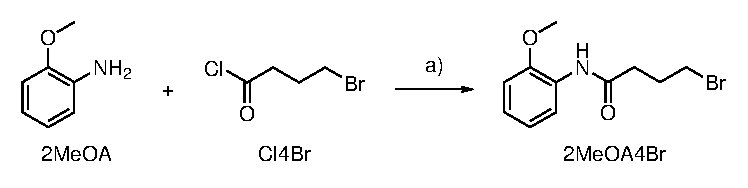
\includegraphics[scale=1]{2MeOA4Br_synth}
		\caption{Synthesis of Br-C$_4$-2-methoxybenzene \compound{cmpd:2MeOA4Br}.
		a) \ce{NaHCO3}, \ce{CH2Cl2}, \ce{H2O}, 0 $^{\circ}$C, 1 h, 50.0 \%.
		\label{sch:2MeOA4Br_synth}}
	\end{center}
\end{scheme}

\subsubsection{Synthesis of the 2-methoxybenzene-CipMe conjugate \compound{cmpd:2MeOA4CipMe}}

The procedure outlined by Ganguly \textit{et al.}\cite{Ganguly2011} was initially attempted in order to synthesise the 2-methoxybenzene-CipMe conjugate \compound{cmpd:2MeOA4CipMe}, but the reaction was very slow and did not go to completion, presumably due to degradation of Br-C$_4$-2-methoxybenzene \compound{cmpd:2MeOA4Br}.
New conditions, employing a microwave reactor and 2 eq. of Br-C$_4$-2-methoxybenzene \compound{cmpd:2MeOA4Br} were then attempted, with a much greater conversion observed by LCMS after 4 h (see \ref{sch:2MeOA4_synth}). However, a poor yield was obtained, possibly due to losses during column chromatography.

\begin{scheme}[H]
	\begin{center}
		\schemeref[2MeOA4Br]{cmpd:2MeOA4Br}
		\schemeref[CipMe]{cmpd:CipMe}
		\schemeref[2MeOA4CipMe]{cmpd:2MeOA4CipMe}
		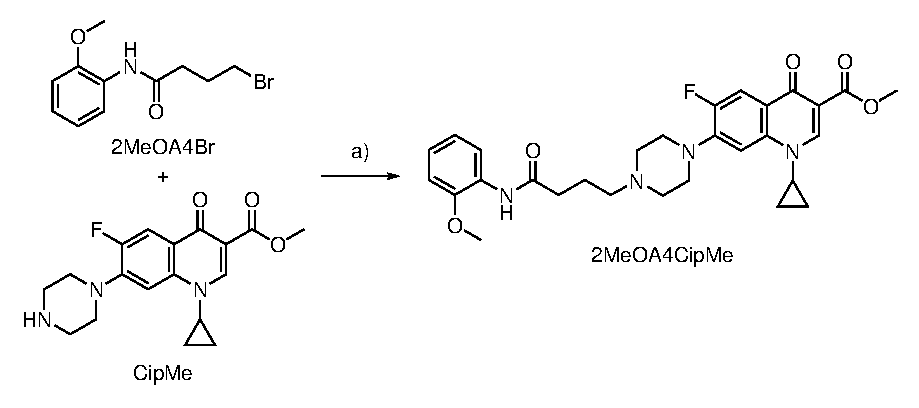
\includegraphics[scale=1]{2MeOA4_synth}
		\caption{Synthesis of the 2-methoxybenzene-CipMe conjugate \compound{cmpd:2MeOA4CipMe}. 
		a) \ce{NaI}, DIPEA, acetonitrile, microwave reactor, 100 $^{\circ}$C, 4 h, 10.2 \%.
		 \label{sch:2MeOA4_synth}}
	\end{center}
\end{scheme}

\subsubsection{Synthesis of the 2-methoxybenzene-Cip triazole conjugate \compound{cmpd:2MeOA4T4Cip}}

\ce{N3}-C$_4$-2-methoxybenzene \compound{cmpd:2MeOA4N3} was synthesised from Br-C$_4$-2-methoxybenzene \compound{cmpd:2MeOA4Br} by an S$_N$2 reaction with sodium azide (see \ref{sch:2MeOA4CipMe_synth}). The yield of \ce{N3}-C$_4$-2-methoxybenzene \compound{cmpd:2MeOA4N3} (26.7 \%) was a lot lower than for \ce{N3}-C$_4$-HCTL \compound{cmpd:SHL4N3} (89.3 \%). However, in this case it may not be better to use the product crude as several impurities were formed during the reaction and could be observed by LCMS (see \ref{fig:2MeOA4N3_impurities}).

\begin{figure}[H]
	\begin{center}
		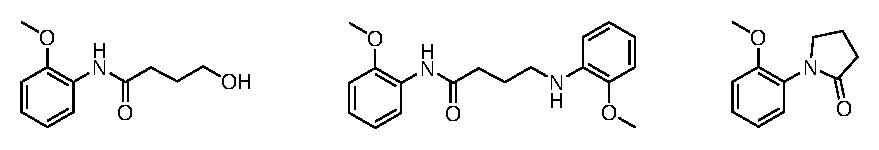
\includegraphics[scale=1]{2MeOA4N3_impurities}
		\caption{Suspected impurities observed by LCMS during the synthesis of \ce{N3}-C$_4$-2-methoxybenzene \compound{cmpd:2MeOA4N3}.
		\label{fig:2MeOA4N3_impurities}}
	\end{center}
\end{figure}

The 2-methoxybenzene-Cip triazole conjugate \compound{cmpd:2MeOA4T4Cip} was synthesised using the standard click conditions  (see \ref{sec:click_general}), with the addition of \ce{CH2Cl2} as a co-solvent to aid the dissolution of \ce{N3}-C$_4$-2-methoxybenzene \compound{cmpd:2MeOA4N3} (see \ref{sch:2MeOA4T4Cip_synth}).

\begin{scheme}[H]
	\begin{center}
		\schemeref[2MeOA4Br]{cmpd:2MeOA4Br}
		\schemeref[2MeOA4N3]{cmpd:2MeOA4N3}
		\schemeref[Y4Cip]{cmpd:Y4Cip}
		\schemeref[2MeOA4T4Cip]{cmpd:2MeOA4T4Cip}		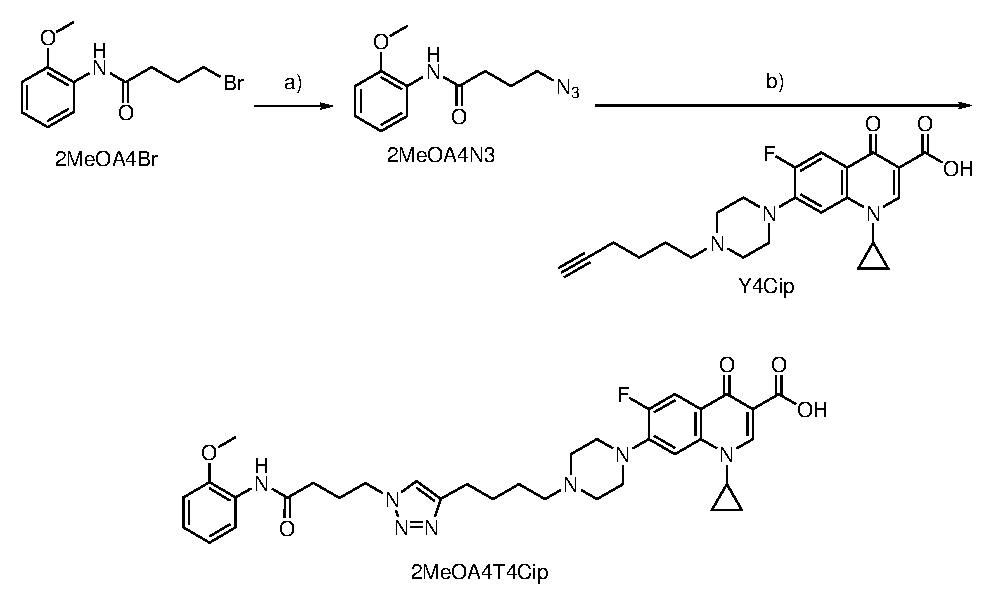
\includegraphics[scale=1]{2MeOA4T4Cip_synth}
		\caption{Synthesis of the 2-methoxybenzene-Cip triazole conjugate \compound{cmpd:2MeOA4T4Cip}. 
		a) \ce{NaN3}, acetonitrile, reflux, 2 h, 26.7 \%. 
		b) \ce{CuSO4}, THPTA, sodium ascorbate, \ce{H2O}, \textit{t}-BuOH, \ce{CH2Cl2}, r.t., 16 h, 39.0 \%.\label{sch:2MeOA4T4Cip_synth}}
	\end{center}
\end{scheme}

\subsection{3-Methoxybenzene derivatives}

\subsubsection{Synthesis of Br-C$_4$-3-methoxybenzene \compound{cmpd:3MeOA4Br}}

Br-C$_4$-3-methoxybenzene \compound{cmpd:3MeOA4Br} was synthesised from 3-methoxyaniline \compound{cmpd:3MeOA} and 4-bromobutyryl chloride \compound{cmpd:Cl4Br} using Schotten-Baumann conditions as above in almost identical (49.6 \%) yield (see \ref{sch:3MeOA4Br_synth}). 

\begin{scheme}[H]
	\begin{center}
		\schemeref[3MeOA]{cmpd:3MeOA}
		\schemeref[Cl4Br]{cmpd:Cl4Br}
		\schemeref[3MeOA4Br]{cmpd:3MeOA4Br}
		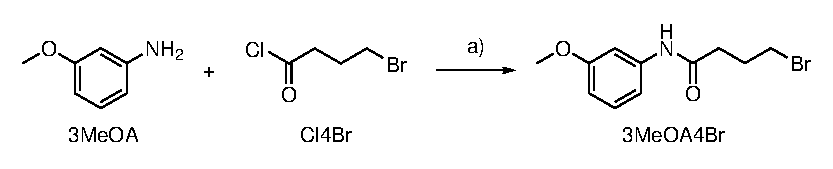
\includegraphics[scale=1]{3MeOA4Br_synth}
		\caption{Synthesis of Br-C$_4$-3-methoxybenzene \compound{cmpd:2MeOA4Br}.
			a) \ce{NaHCO3}, \ce{CH2Cl2}, \ce{H2O}, 0 $^{\circ}$C, 1 h, 49.6 \%. \label{sch:3MeOA4Br_synth}}
	\end{center}
\end{scheme}

\subsubsection{Synthesis of the 3-methoxybenzene-CipMe conjugate \compound{cmpd:3MeOA4CipMe}}

The 3-methoxybenzene-CipMe conjugate \compound{cmpd:3MeOA4CipMe}, 
was synthesised as above, in similar yield (see \ref{sch:3MeOA4_synth}).

\begin{scheme}[H]
	\begin{center}
		\schemeref[3MeOA4Br]{cmpd:3MeOA4Br}
		\schemeref[CipMe]{cmpd:CipMe}
		\schemeref[3MeOA4CipMe]{cmpd:3MeOA4CipMe}
		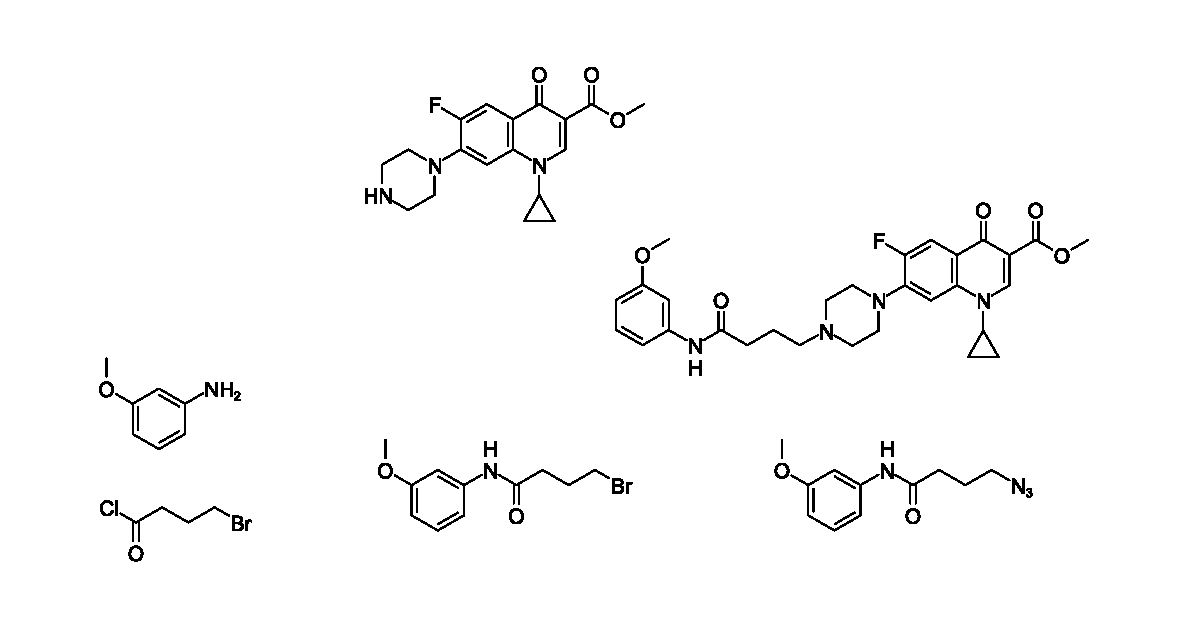
\includegraphics[scale=1]{3MeOA4_synth}
		\caption{Synthesis of the 3-methoxybenzene-CipMe conjugate \compound{cmpd:3MeOA4CipMe}. 
		a)  \ce{NaI}, DIPEA, acetonitrile, microwave reactor, 100 $^{\circ}$C, 4 h, 10.5 \%.
		\label{sch:3MeOA4_synth}}
	\end{center}
\end{scheme}

\subsubsection{Synthesis of the 3-methoxybenzene-Cip triazole conjugate \compound{cmpd:3MeOA4T4Cip}}

\ce{N3}-C$_4$-2-methoxybenzene \compound{cmpd:2MeOA4N3} 
and the 3-methoxybenzene-Cip triazole conjugate \compound{cmpd:3MeOA4T4Cip} were synthesised as above, in similar yields (see \ref{sch:3MeOA4_synth} and \ref{sch:3MeOA4T4Cip_synth}).

\begin{scheme}[H]
	\begin{center}
		\schemeref[3MeOA4Br]{cmpd:3MeOA4Br}
		\schemeref[3MeOA4N3]{cmpd:3MeOA4N3}
		\schemeref[Y4Cip]{cmpd:Y4Cip}
		\schemeref[3MeOA4T4Cip]{cmpd:3MeOA4T4Cip}		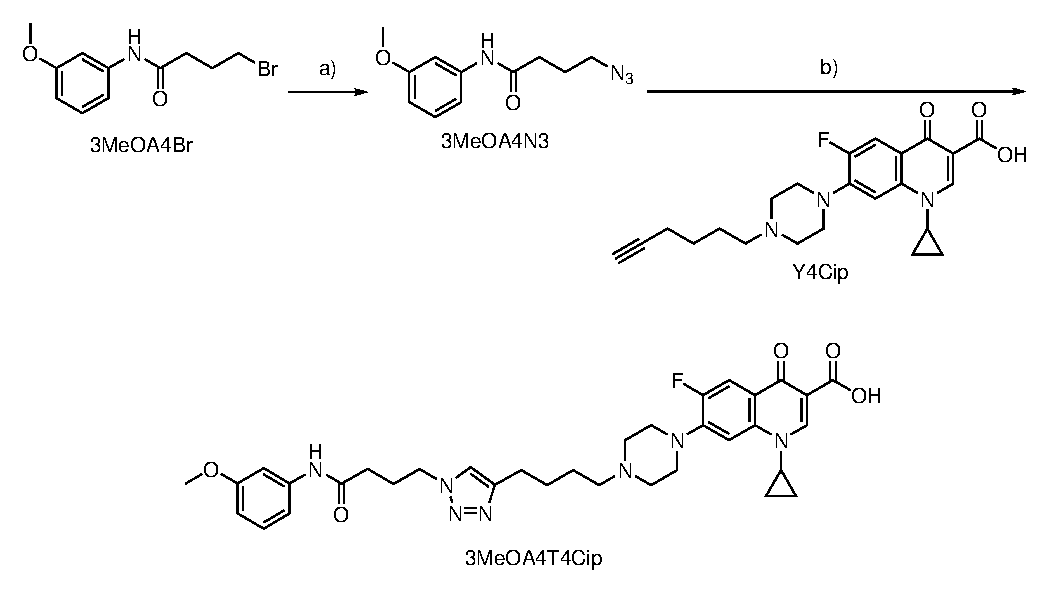
\includegraphics[scale=1]{3MeOA4T4Cip_synth}
		\caption{Synthesis of the 3-methoxybenzene-Cip triazole conjugate \compound{cmpd:3MeOA4T4Cip}. 
		a) \ce{NaN3}, acetonitrile, reflux, 7 h, 16.7 \%. 
		b) \ce{CuSO4}, THPTA, sodium ascorbate, \ce{H2O}, \textit{t}-BuOH, \ce{CH2Cl2}, r.t., 2 h, 5.0 \%. 
		\label{sch:3MeOA4T4Cip_synth}}
	\end{center}
\end{scheme}

